\documentclass[a4paper, 12pt]{article}
\usepackage[utf8]{inputenc}
\usepackage[T1]{fontenc}
\usepackage{amsmath}
\usepackage{amsfonts}
\usepackage{amssymb}
\usepackage{amsthm}
\usepackage[top=2cm, bottom=3cm, left=3cm, right=3cm]{geometry}
\usepackage{graphicx}
\usepackage[table]{xcolor}
\usepackage{tikz}
\usetikzlibrary{intersections, angles, quotes, shapes.multipart}
\usepackage{microtype}
\usepackage{array}
\usepackage{tabularx}
\usepackage{enumitem}
\usepackage{fancyhdr}
\usepackage{hyperref}
\usepackage{algorithmic}
\usepackage{ifthen}
\usepackage{listofitems}
\usepackage{xstring}
\usepackage{anyfontsize}
\usepackage{float}
\usepackage{multicol}
\usepackage{listings}
\setlength{\headheight}{15pt}
\addtolength{\topmargin}{15.8546pt}
\pagestyle{fancy}
\lhead{\today}
\chead{}
\rhead{\includegraphics[width=1.5cm]{Logo/logoitts.png}\includegraphics[width=1.2cm]{Logo/IF.jpg}}
\lfoot{Judul Tugas}
\cfoot{}
\rfoot{Halaman \thepage}

\renewcommand{\headrulewidth}{0.4pt}
\renewcommand{\footrulewidth}{0pt}

\newtheorem{theorem}{Theorem}
\newtheorem{lemma}{Lemma}
\newtheorem{definition}{Definition}

\theoremstyle{definition}
\newtheorem{soal}{Soal}

\theoremstyle{remark}
\newtheorem*{solution}{Solution}
\newtheorem*{remark}{Remark}
\renewcommand\qedsymbol{$\blacksquare$}

\lstset{
    language=C++, 
    basicstyle=\ttfamily\small,
    aboveskip={1.0\baselineskip},
    belowskip={1.0\baselineskip},
    columns=fixed,
    extendedchars=true,
    breaklines=true,
    tabsize=4,
    prebreak=\raisebox{0ex}[0ex][0ex]{\ensuremath{\hookleftarrow}},
    frame=lines,
    showtabs=false,
    showspaces=false,
    showstringspaces=false,
    keywordstyle=\color[rgb]{0.627,0.126,0.941},
    commentstyle=\color[rgb]{0.133,0.545,0.133},
    stringstyle=\color[rgb]{01,0,0},
    backgroundcolor=\color{gray!10},
    numbers=left,
    numberstyle=\small,
    stepnumber=1,
    numbersep=10pt,
    captionpos=t,
    escapeinside={\%*}{*)}
}

\lstset{
    language=Python, 
    basicstyle=\ttfamily\small,
    aboveskip={1.0\baselineskip},
    belowskip={1.0\baselineskip},
    columns=fixed,
    extendedchars=true,
    breaklines=true,
    tabsize=4,
    prebreak=\raisebox{0ex}[0ex][0ex]{\ensuremath{\hookleftarrow}},
    frame=lines,
    showtabs=false,
    showspaces=false,
    showstringspaces=false,
    keywordstyle=\color[rgb]{0.627,0.126,0.941},
    commentstyle=\color[rgb]{0.133,0.545,0.133},
    stringstyle=\color[rgb]{01,0,0},
    backgroundcolor=\color{gray!10},
    numbers=left,
    numberstyle=\small,
    stepnumber=1,
    numbersep=10pt,
    captionpos=t,
    escapeinside={\%*}{*)}
}
\setlength\parindent{0pt}

\begin{document}
{\bf Course Code - Course Name}
{\centering
\rule{150mm}{0.15cm}\\[0.5cm]
\fontsize{30}{30} {\bf Tugas $N$}\\[0.3cm]
\rule{150mm}{0.05cm}\\[0.5cm]
}
\begin{tabular}{ll}
Nama & : Ahmad Mu'min Faisal\\
NIM & : 1202210029\\
Kelas & : IF - 01 - 01
\end{tabular}
\hfill
\begin{tabular}{ll}
Prodi & : Informatika\\
Tanggal & : 8 Maret 2022\\
E-mail & : \href{mailto:ahmad.faisalewy@gmail.com}{\textcolor{blue}{ahmad.faisalewy@gmail.com}}
\end{tabular}

\vspace*{.4cm}
{\centering
\rule{150mm}{0.15cm}\\[0.5cm]
}




 
\thispagestyle{empty}
\section{Programming Needs}
\begin{soal}[Lampu dan Tombol]
    Soal ini diambil dari buku Pemrograman Kompetitif Dasar \cite{PKD}.
    \begin{center}
    Batas waktu: 1 detik\\
    Batas memori: 64 MB
    \end{center}
    Terdapat $N$ tombol yang dinomori dari $1$ hingga $N$ dan sebuah lampu dalam keadaan mati. Apabila tombol ke-$i$ ditekan, keadaan lampu akan berubah (dari mati menjadi menyala, atau sebaliknya) apabila $N$ habis dibagi oleh $i$. Apabila masing-masing tombol ditekan tepat sekali, bagaimana keadaan lampu pada akhirnya?
    
    \vspace{12pt}
    \textbf{Format Masukan}
    
    Sebuah baris berisi sebuah bilangan, yaitu $N$.
    
    \vspace{12pt}
    \textbf{Format Keluaran}\\
    Sebuah baris berisi:
    \begin{itemize}
        \item "lampu mati", apabila keadaan akhir lampu adalah mati.
        \item "lampu menyala", apabila keadaan akhir lampu adalah menyala.
    \end{itemize}
    
    \textbf{Contoh Masukan 1}
    
    $5$
    
    \vspace{12pt}
    \textbf{Contoh Keluaran 1}
    
    lampu mati
    
    \vspace{12pt}
    \textbf{Contoh Masukan 2}
    
    $4$
    
    \vspace{12pt}
    \textbf{Contoh Keluaran 2}
    
    lampu menyala
    
    \vspace{12pt}
    \textbf{Penjelasan}
    
    Pada contoh pertama, tombol yang mempengaruhi keadaan lampu adalah tombol
    1 dan tombol 5. Penekanan tombol 1 mengakibatkan lampu menjadi menyala, dan penekanan tombol 5 mengembalikannya ke keadaan mati.
    Pada contoh kedua, tombol yang mempengaruhi keadaan lampu adalah tombol 1, tombol 2, dan tombol 4. Penekanan tombol 1 mengakibatkan lampu menjadi menyala, penekanan tombol 2 mengembalikannya ke keadaan mati, dan penekanan tombol 4 menjadikan lampu kembali menyala.
    
    \vspace{12pt}
    \textbf{Batasan}
    \begin{itemize}
        \item $1\leq N \leq 10^{18}$
    \end{itemize}
\end{soal}

    \begin{solution} Perhatikan bahwa kita tidak perlu tahu berapa banyak pembagi bilangan $N$. Kita hanya perlu tahu apakah $N$ memiliki pembagi sebanyak ganjil atau genap.
    
    Jika suatu bilangan, sebut saja $x$ membagi habis $N$, maka otomatis $\frac{N}{x}$ juga akan membagi habis $N$. Perhatikan contoh berikut:
    
    Jika $N$ = 12, maka:
    \begin{itemize}
        \item Karena $1$ membagi habis $12$, maka $\frac{12}{1} = 12$ juga membagi habis $12$.
        \item Karena $2$ membagi habis $12$, maka $\frac{12}{2} = 6$ juga membagi habis $12$.
        \item Karena $3$ membagi habis $12$, maka $\frac{12}{3} = 4$ juga membagi habis $12$
    \end{itemize}
    
    Dengan demikian, secara umum pembagi bilangan selalu memiliki pasangan, kecuali
    jika $N$ merupakan bilangan kuadrat, misalnya $4,9,16$ dan seterusnya. Mengapa demikian? Jika $N$ merupakan bilangan kuadrat, artinya $N$ dapat dibagi habis oleh $\sqrt{N}$. Khusus pembagi
    akar ini tidak memiliki pasangan, karena $\frac{N}{\sqrt{N}}=\sqrt{N}$. Perhatikan contoh berikut:
    
    Jika $N = 16$, maka:
    \begin{itemize}
        \item Karena $1$ membagi habis $16$, maka $\frac{16}{1} = 16$ juga membagi habis $16$.
        \item Karena $2$ membagi habis $16$, maka $\frac{16}{2} = 8$ juga membagi habis $16$.
        \item $4$ membagi habis $16$, tetapi karena $\frac{16}{4}$ juga $4$ , maka pembagi ini tidak memiliki pasangan.
    \end{itemize}

    Maka kita bisa simpulkan bahwa lampu menyala jika dan hanya jika $N$ merupakan bilangan kuadrat. Untuk menentukan apakah $N$ merupakan bilangan kuadrat, kita dapat menghitung pembulatan dari $\sqrt{N}$, sebut saja $s$. Kemudian menghitung $s\times s$ lagi. Jika kita
    mendapatkan kembali $N$, maka $N$ adalah bilangan kuadrat.
    
    Sebagai contoh:
    \begin{itemize}
        \item $N = 8$, maka $\sqrt{8} \approx 2.828427$, dibulatkan menjadi $3$. Hasil dari $3\times 3$ bukan $8$, maka $8$ bukan bilangan kuadrat.
        \item $N = 9$, maka $\sqrt{9} = 3$, dibulatkan menjadi $3$. Hasil dari $3\times 3$ adalah $9$, maka $9$ adalah bilangan kuadrat.
        \item $N = 10$, maka $\sqrt{10} \approx 3.162277$, dibulatkan menjadi $3$. Hasil dari $3\times 3$ bukan $10$, maka $10$ bukan bilangan kuadrat
    \end{itemize}
    
    \begin{lstlisting}[label={list:first},caption=Solusi dalam bahasa C++]
    #include<iostream>
    #include<cmath>
    
    using namespace std;
    
    int main(){
        long long N;
        cin >> N;
        long long s = round(sqrt(N));
        if(s * s != N){
            cout << "lampu mati" << endl;
        }
        else{
            cout << "lampu menyala" << endl;
        }
    }
    \end{lstlisting}
\end{solution}

\section{Mathematical Needs}

\begin{theorem}[Division Algorithm]
    For every integer pair $a, b$, there exists distinct integer quotient and remainder, $q$ and $r$, that satisfy
    \[a=bq+r,\ 0\leq r< n\]
\end{theorem}
\begin{proof}
    We will prove that this is true for when a and b are positive. The other
cases when one or both of $a$ and $b$ are negative follow very similarly. There are
two parts in this proof:
\begin{itemize}
    \item Proving that for every pair $(a, b)$ we can find a corresponding quotient and
    remainder.
    \item Proving that this quotient and remainder pair are unique.

\end{itemize}
For proving the existence of the quotient and remainder, given two integers $a$
and $b$ with varying $q$, consider the set
\[\{a - bq\ \text{with}\ q\ \text{an integer and}\ a - bq \geq 0\}.\]

By the well-ordering principle we know that this set must have a minimum, say
when $q = q_1$. Clearly from the condition on the set, we must have $a-bq_1 = r \geq 0$.
It now serves to prove that $a - bq_1 = r < b$. For the sake of contradiction, assume
that $a - bq_1 \geq b$. However, then
\[a - b(q_1 + 1) \geq 0,\]
therefore it also should be a member of the above set. Furthermore,
\[a - b(q_1 + 1) < a - bq_1,\]
contradicting the minimality of $q_1$. Therefore, it is impossible for $a-bq_1 \geq b$, and
we have $0 \leq a - bq_1 < b$.

The second part of this proof is to show that the quotient and remainder are
unique. Assume for the sake of contradiction that a can be represented in two
ways:
\begin{align*}
    a = bq_1 + r_1 &= bq_2 + r_2\\
    b(q_1 - q_2) &= r_2 - r_1.
\end{align*}
This implies that $b | r_2 - r_1$. However,
\[b > r_2 - r_1 > -b\]
since $0 \leq r_1, r_2 < b$. Since $r_2 - r_1$ is a multiple of $b$, we must have $r_2 - r_1 = 0 \Rightarrow
r_2 = r_1\ \text{and}\ q_2 = q_1$ \cite{NTJS3}.
\end{proof}

\section{How To Draw an Image Using TikZ}
\begin{center}
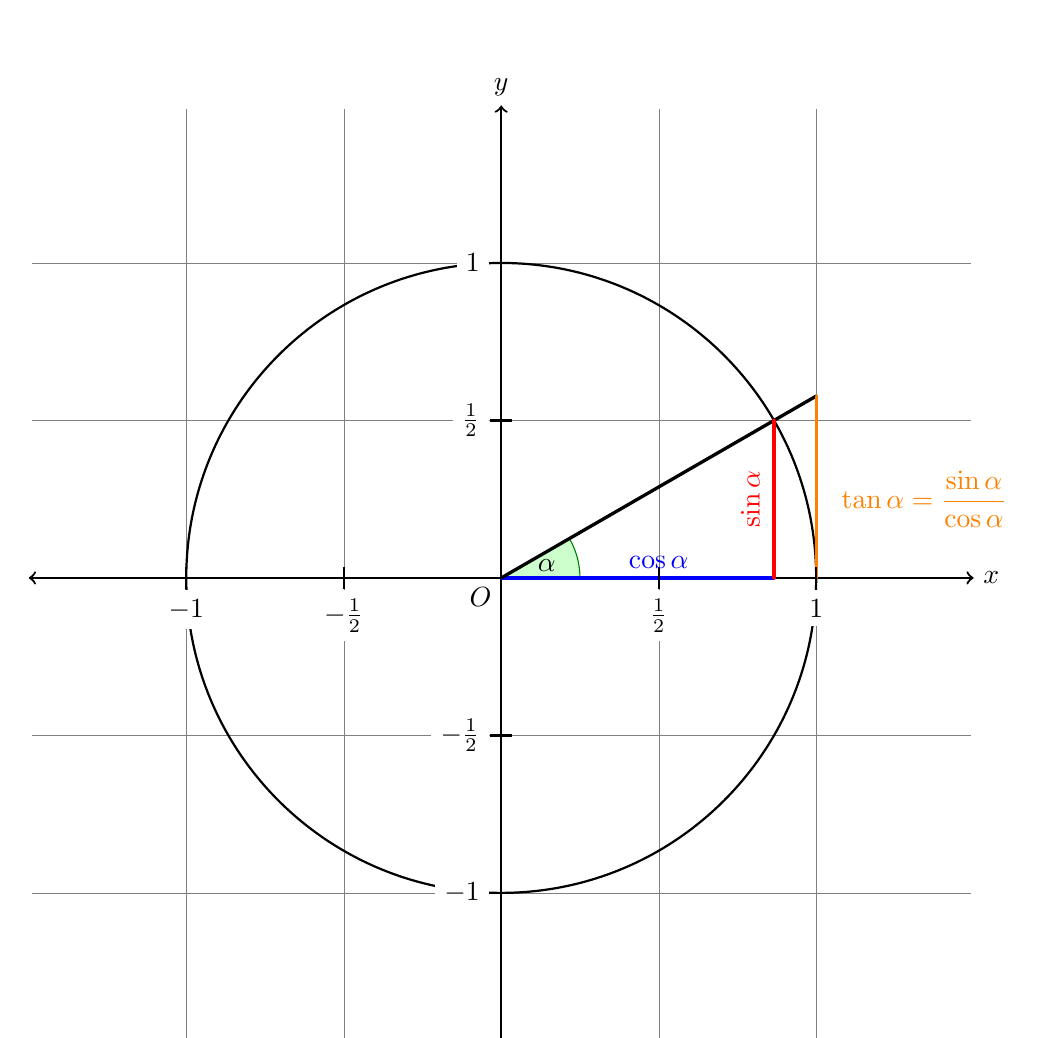
\begin{tikzpicture}[scale=4]
    \coordinate (O) at (0,0) node[anchor=north east]{$O$};
    \coordinate (x1) at (-1.5,0);
    \coordinate[label=right:$x$] (x2) at (1.5,0);
    \coordinate (y1) at (0,-1.5);
    \coordinate[label=above:$y$] (y2) at (0,1.5);
    \coordinate (A) at (1,0);
    \coordinate (C) at (30:1cm);
    \coordinate (P) at (1, {tan(30)});
    \draw[gray, ultra thin, step=.5cm] (-1.49,-1.49) grid (1.49,1.49);
    \draw[thick, <->] (x1)--(x2);
    \draw[thick, <->] (y1)--(y2);
    \draw[thick] (O) circle[radius=1];
    \draw pic [draw=green!50!black, fill=green!20, angle                radius=10mm,"$\alpha$"] {angle = A--O--C};
    \draw[blue,very thick, line cap=round] (30:1cm) ++(0,-0.5) -- (0,0);
    \draw[very thick, line cap=round] (O)--(P);
    \draw[red, very thick, line cap=round] (30:1cm)-- +(0,-.5);
    \draw[orange, very thick, line cap=round] (1,{tan(30)})--(1,0);
    \foreach \x/\xtext in {-1,-.5/-\frac{1}{2},.5/\frac{1}{2},1}
        \draw[thick] (\x,1pt)--(\x,-1pt) node[fill=white, below]{$\xtext$};
    \foreach \y/\ytext in {-1,-0.5/-\frac{1}{2},0.5/\frac{1}{2},1}
        \draw[thick] (1pt,\y)--(-1pt,\y) node[fill=white, left]{$\ytext$};
    \node[orange, right] at (1.05, 0.25) {$\displaystyle{\tan{\alpha}=\frac{\sin{\alpha}}{\cos{\alpha}}}$};
    \node[red, rotate=90] at ({cos(30)-0.075}, 0.25) {$\sin{\alpha}$};
    \node[blue, above] at (1/2, 0){$\cos{\alpha}$};
\end{tikzpicture}
\end{center}

\bibliographystyle{IEEEtran}
\bibliography{Referensi.bib}

\end{document}
